\documentclass[border=5pt]{standalone}
\usepackage[T1]{fontenc}
\usepackage{amsmath,amssymb,tikz,xcolor}
\usetikzlibrary{arrows.meta,positioning,calc}
\definecolor{ink}{HTML}{243B53}
\definecolor{signal}{HTML}{087F8C}
\definecolor{command}{HTML}{D87525}
\definecolor{pale}{HTML}{EEF4F8}
\tikzset{
 pics/radio/.style={code={
  \draw[ink,line width=1.2pt] (0,.5)--(-.34,-.52)--(.34,-.52)--cycle;
  \draw[ink,line width=.8pt] (-.19,-.08)--(.19,-.08) (-.27,-.32)--(.27,-.32);
  \fill[signal] (0,.57) circle (.065);
  \draw[signal,line width=1pt] (-.22,.38) arc[start angle=220,end angle=140,radius=.29]
   (.22,.38) arc[start angle=-40,end angle=40,radius=.29];
  \draw[signal,line width=1pt] (-.42,.23) arc[start angle=220,end angle=140,radius=.54]
   (.42,.23) arc[start angle=-40,end angle=40,radius=.54];
  \draw[ink,line width=.8pt,rounded corners=1pt] (-.94,-.48) rectangle (-.65,.05);
  \draw[signal,line width=.7pt] (-.89,-.34)--(-.70,-.34);
 }},
 pics/router/.style={code={
  \path[fill=pale,draw=ink,line width=1pt] (-.7,-.27)--(.5,-.27)--(.76,-.04)--(-.44,-.04)--cycle;
  \path[fill=white,draw=ink,line width=1pt] (-.7,-.27)--(.5,-.27)--(.5,-.60)--(-.7,-.60)--cycle;
  \path[fill=ink!12,draw=ink,line width=1pt] (.5,-.27)--(.76,-.04)--(.76,-.37)--(.5,-.60)--cycle;
  \foreach \x in {-.53,-.31,-.09,.13}{\draw[ink,line width=.65pt] (\x,-.36) rectangle +(0.13,-.12);}
  \draw[signal,->,line width=1pt] (-.15,.14)--(-.65,.14);
  \draw[signal,->,line width=1pt] (.15,.34)--(.65,.34);
  \draw[signal,->,line width=1pt] (0,.24)--(0,.72);
 }},
 pics/server/.style={code={
  \path[fill=ink!10,draw=ink,line width=.8pt] (.43,-.65)--(.67,-.47)--(.67,.61)--(.43,.43)--cycle;
  \path[fill=pale,draw=ink,line width=.8pt] (-.48,.43)--(-.24,.61)--(.67,.61)--(.43,.43)--cycle;
  \foreach \y in {-.48,-.1,.28}{
   \path[fill=white,draw=ink,rounded corners=1pt,line width=.9pt] (-.48,\y-.17) rectangle (.43,\y+.17);
   \fill[signal] (-.32,\y) circle (.045);
   \draw[ink!55,line width=.7pt] (-.15,\y)--(.26,\y);
  }
 }},
 pics/control/.style={code={
  \path[fill=white,draw=ink,line width=1pt,rounded corners=2pt] (-.65,-.3) rectangle (.65,.5);
  \draw[ink,line width=1pt] (0,-.3)--(0,-.55) (-.32,-.55)--(.32,-.55);
  \draw[signal,line width=1.1pt] (-.46,-.05)--(-.22,.18)--(.02,.06)--(.23,.32)--(.43,.22);
  \foreach \x/\y in {-.46/-.05,-.22/.18,.02/.06,.23/.32,.43/.22}{\fill[signal] (\x,\y) circle (.035);}
 }},
 pics/report/.style={code={
  \path[fill=white,draw=ink,line width=.9pt,rounded corners=1pt] (-.43,-.57) rectangle (.43,.57);
  \draw[ink!40,line width=.8pt] (-.26,.32)--(.22,.32) (-.26,.15)--(.08,.15);
  \fill[signal!40] (-.26,-.37) rectangle (-.14,-.11);
  \fill[signal!65] (-.04,-.37) rectangle (.08,-.02);
  \fill[signal] (.18,-.37) rectangle (.30,.16);
 }},
 pics/memory/.style={code={
  \foreach \y in {-.37,0,.37}{
   \path[fill=white,draw=ink,line width=.9pt,rounded corners=1pt] (-.57,\y-.13) rectangle (.57,\y+.13);
   \fill[command] (-.39,\y) circle (.04);
   \draw[ink!50,line width=.7pt] (-.21,\y)--(.37,\y);
  }
 }},
 pics/clock/.style={code={
  \draw[command,line width=1pt,fill=white] (0,0) circle (.4);
  \draw[command,line width=1pt] (0,.26)--(0,0)--(.19,-.12);
 }}
}


\begin{document}
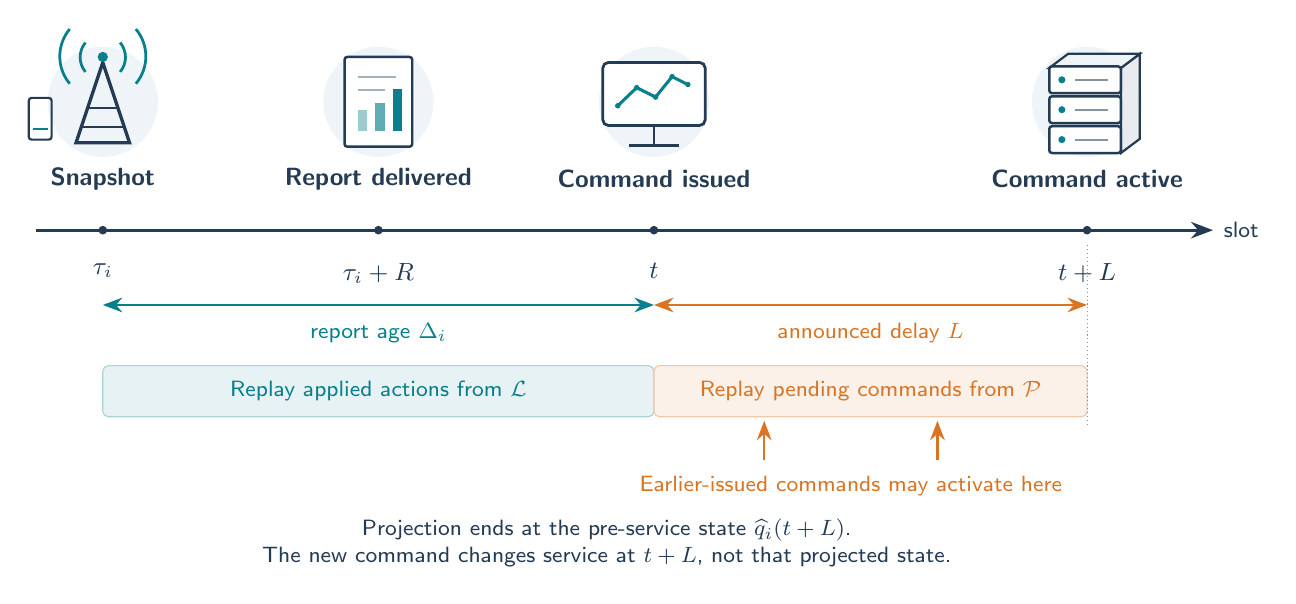
\begin{tikzpicture}[>=Stealth,x=1cm,y=1cm,font=\small\sffamily]
% Four event landmarks use the same icon vocabulary as the architecture.
\foreach \x in {1,4.5,8,13.5}{\path[fill=pale,draw=none] (\x,3.25) circle (.7);}
\pic at (1,3.25) {radio};
\pic at (4.5,3.25) {report};
\pic at (8,3.25) {control};
\pic at (13.5,3.25) {server};
\node[font=\small\sffamily\bfseries,text=ink] at (1,2.27){Snapshot};
\node[font=\small\sffamily\bfseries,text=ink] at (4.5,2.27){Report delivered};
\node[font=\small\sffamily\bfseries,text=ink] at (8,2.27){Command issued};
\node[font=\small\sffamily\bfseries,text=ink] at (13.5,2.27){Command active};
\draw[->,ink,line width=1.1pt] (.15,1.62)--(15.1,1.62) node[right,font=\footnotesize\sffamily]{slot};
\foreach \x/\lab in {1/{$\tau_i$},4.5/{$\tau_i+R$},8/{$t$},13.5/{$t+L$}}{
 \fill[ink] (\x,1.62) circle (.055);
 \node[below=3mm,text=ink] at (\x,1.62){\lab};
}
\draw[<->,signal,line width=.9pt] (1,.67)--node[below=1mm,font=\footnotesize\sffamily]{report age $\Delta_i$}(8,.67);
\draw[<->,command,line width=.9pt] (8,.67)--node[below=1mm,font=\footnotesize\sffamily]{announced delay $L$}(13.5,.67);
\path[fill=signal!10,draw=signal!35,rounded corners=2pt] (1,-.75) rectangle (8,-.10);
\path[fill=command!10,draw=command!40,rounded corners=2pt] (8,-.75) rectangle (13.5,-.10);
\node[text=signal,font=\footnotesize\sffamily] at (4.5,-.42){Replay applied actions from $\mathcal L$};
\node[text=command,font=\footnotesize\sffamily] at (10.75,-.42){Replay pending commands from $\mathcal P$};
\foreach \x in {9.4,11.6}{\draw[->,command,line width=.9pt] (\x,-1.3)--(\x,-.8);}
\node[text=command,font=\footnotesize\sffamily] at (10.5,-1.63){Earlier-issued commands may activate here};
\draw[densely dotted,ink!55] (13.5,-.85)--(13.5,1.45);
\node[align=center,font=\footnotesize\sffamily,text=ink] at (7.4,-2.35)
 {Projection ends at the pre-service state $\widehat q_i(t+L)$.\\The new command changes service at $t+L$, not that projected state.};
\end{tikzpicture}
\end{document}
